\documentclass[nojss]{jss}
\usepackage[latin1]{inputenc}
\graphicspath{{Figures/}}

%% for internal use
\newcommand{\fixme}[1]{\emph{\marginpar{FIXME} (#1)}}
\newcommand{\readme}[1]{\emph{\marginpar{README} (#1)}}


\title{Something about Euro, EMU, and Inflation}

% Verkaufsstrategien
% 1. Widerlegung des Teuro Effektes
% 2. Keine Ver�nderung d. EMU sichtbar; nach 2002 kein globaler Trend aller EMU Staaten Richtung Wechsel
% 3. Nutzen zeigen, den die osteurop�ischen Staaten haben, dadurch, dass sie dem EURO beitreten m�ssen
%    (mit Ausnahme von Slovenien fallender Trend in Mittelwert und Varianz)
%    so etwa in Slowenien und der Slovakei ein Bruch bevor diese Staaten dem ERMII/EURO beitreten
% 4. Finanzkrise: schwieriger, ausser Irland keine �nderung > 2008


% Loswerden der Working Papers
% auf Zitat mit castelnuovo kann man verzichten, dass die EZB Preisstabilit�t so
% definiert ist kein Geheimenis und nichts, dass man mit Paper zitieren m�sste
% Z: Bitte das offizielle ECB-Statement zitieren

% holem�ller geht nicht weg, immer noch Discussion Paper (siehe sein
% lebenslauf) http://www.holtem.de/Dokumente/PublicCV-Holtemoeller.pdf
% morana detto
% Z: Das ist ok, ein paar Working Papers koennen schon bleiben.
%    Aber: @TechReport nicht @Article benutzen (schon erledigt)

\author{Thomas Windberger\\Universit\"at Innsbruck \And
        Achim Zeileis\\Universit\"at Innsbruck
}
\Plainauthor{Thomas Windberger, Achim Zeileis}

\Abstract{
  The aim of this paper is to shed some light on the effect of the economic and monetary union
  on changing the volatility of the inflation rates in the member states of the European Union. 
}

\Keywords{inflation rate, structural break, EMU}


\Address{
  Thomas Windberger, Achim Zeileis\\
  Department of Statistics\\
  Universit\"at Innsbruck\\
  Universit\"atsstra�e 15\\
  6020 Innsbruck, Austria\\
  E-mail: \email{Thomas.Windberger@student.uibk.ac.at}, \email{Achim.Zeileis@R-project.org}
}


\begin{document}


\section{Introduction}

The European Central Bank (ECB) defines price stability ``as a year-on-year
increase in the Harmonized Index of Consumer Prices (HICP) for the Euro area of
below 2\%''. \fixme{some official ECB reference needed for quote}
\citet{emerson} emphasize the fact that a high inflation rate is
also more variable and uncertain and thus causes more relative price
variability, leading to a less efficient price mechanism (p.~22).
% Therefore a vital aim of every central bank is to achieve a low inflation rate
% with negligible variation.
The question of interest centers around the way in which a country's decision to
join the economic and monetary union (EMU) \readme{Note that the E in EMU stands for economic, not European}
changed its inflation rate dynamics. 

% There are a number of reasons why these should have changed indeed. Given
% that a country experienced quite volatile inflation rates, its efforts to meet the
% convergence criteria were likely to lead to an alternation at least in the mean
% (since this was required for a number of countries) and possible in the
% volatility of their respective inflation rates as well. This has indeed been the
% case for a host of EMU countries, like Spain, Italy and Portugal, reflecting
% their effort to meet the Maastricht Criteria for inflation rates.
% no literature overview

Theory unfortunately is quite unsure  whether or not the creation of a monetary
union between two or more states is likely to reduce or increase the variability
or even the level of the inflation rate.  \citet{cooper} point out, that ``a
central bank under a monetary union will internalize the interdependence between
countries and optimally choose a lower inflation rate" and argue that a
``central bank governing the growth of money supply will optimally choose zero
inflation." This is not the case with the ECB which targets 2\% so as to
avoid the risk of deflation. Thus, it is not quite clear how a monetary union
will affect the volatility and the level of the inflation rate.

An interesting approach to this question is taken by \citet{holte}. 
% He creates a two country model for monetary policy analysis along the line of
% two models by \citet{mc1} and \citet{mc2} as well as \citet{gali}. The inflation
% is modeled by a hybrid Phillips curve  specification and there are a number of
% different home country interest rate rules, like strict inflation targeting,
% flexible targeting, pegging to a currency and --  monetary union. 
What he finds out via simulations of  different interest rate rules is that the
standard deviation of the home consumer price index (CPI) inflation rate can be substantially reduced
by joining a monetary union.
% But monetary policy in a monetary union does not explicitly stabilize the
% output gap and inflation rate in case of national economic shocks. 
The effects of joining a monetary union on inflation rate variability depend on
structural parameters like risk aversion, price flexibility, export demand
elasticity, openness and shock correlations. Due to the fact that not all of
these parameters are known and that their interaction as well has to be
estimated, theory has some troubles establishing a sound theoretical model.

\citet{cap} estimate short-run and steady-state inflation uncertainty in 12 EMU
countries and find a considerable degree of heterogeneity across EMU countries
in terms of average inflation and its degree of persistence.
% They use a time-varying model with a GARCH specification for the unconditional
% volatility of inflation and find some instability in the conditional volatility.


In a paper examining structural convergence of the inflation rates in EU
countries, \citet{palomba} try to answer the question whether during the 1990s the
inflation rate dynamics of EU countries became more similar. They find that
there is only partial evidence for convergence in time of inflation dynamics.  In a
paper studying core inflation and using an aggregated Euro area inflation rate,
\citet{morana} finds three regimes (roughly 1980---1984, 1984---1993 and
1993---2000) governing the core inflation rate.

Inquiring into the
convergence properties of inflation rates among countries of the EMU,
\citet{busetti} find that from 1980---1997 there was convergence of inflation
rates, but afterwards there is some diverging behavior.


\section{Data}

Inflation is measured as the logarithm of the monthly change in the HICP from
January 1990 to March 2010. Countries included are Austria, Belgium, the Czech
Republic, Denmark, Estonia, Finland, France, Germany, Greece, Hungary, Ireland,
Italy, Luxembourg, The Netherlands, Poland, Portugal, Spain, Sweden, and the
United Kingdom.  The data are obtained from the OECD Statistics \fixme{It would be
good to cite something here. Is there some stable reference/link for the OECD data source?}.
Latvia, Lithuania, Bulgaria, and Romania are excluded due to data scarcity.

The countries can be divided into three different groups. (1)~The Euro countries:
Austria, Belgium, Estonia (which will enter in 2011), France,
Finland, Germany, Greece, Ireland, Italy, Luxembourg, The Netherlands, Portugal,
Spain and Slovenia.\footnote{Cypria, Malta, Andorra, Monaco, San Marino and the
Vatican are left out due their minor importance.} (2)~EU members without ERM~II
(exchange rate mechanism): Czech Republic, Hungary, Poland, Sweden, and the United
Kingdom. Denmark stands on its own as a member of the EU and the
ERM~II, but not yet a member of the EMU.

\section{Methods}

\subsection{A Generalized Logistic Distribution}

In econometrics, the logistic distribution is often used in income distributions and growth models. This is due to  its longer tails and  higher peak, which fits these problems somewhat better. The use of the generalized logistic distribution as we will use it in this paper is rather rare. \citet{won} uses a GL distribution in a regression model with autocorrelated errors and assumes that they follow a GL distribution rather than a Student's t-distribution, as to model the fact that these are oftentimes  leptokurtic and severely left or right skewed. A similar GL distribution is also used in \citet{tolikas} who analyses extreme risk and value--at--risk in the German stock market, all though they don't use a shape parameter. Regarding inflation rates, the GL distribution is --- to our best knowledge --- only used in relationship with expected inflation. \citet{batchelor} use a logistic distribution (not its generalization) to model the distribution of mean expected inflation rates. 

We apply the general framework, as developed in \citet{z07}, to a more specific model, in this case by means of a GL distribution. Prior to that, we would like to give a short justification for the usage of the GL distribution. Regarding the data at hand, it was not possible to use the already existing method developed in \citet{z07}, since almost all inflation rates, with the notable exception of Greece, are not normally distributed and clearly exhibit asymmetric properties. 

Therefore, a somewhat more flexible distribution had to be used. We needed a distribution exhibiting rather strong kurtosis and the property to be both left and right skewed. To serve this purpose, we use a generalization of the logistic distribution as defined in \citet{johnson}. Its probability density is given by:
%
\begin{eqnarray}
f(\pi | \theta, \sigma, \delta) & = & \frac{\frac{\delta}{\sigma}*\exp^{-\frac{\pi_i-\theta}{\sigma}}}{(1+\exp^{-\frac{\pi_i-\theta}{\sigma}})^{(\delta+1)}}
\end{eqnarray}
%
with location ($\theta$), scale ($\sigma$) and shape ($\delta$). For b=1 the distribution simplifies to the logistic distribution, for b$<$1 it is skewed to the left and for b$>$1 it is skewed to the right. The moments are given by:
%
\begin{eqnarray}
E(\pi_i) & = & \theta + \sigma (\gamma(\delta) - \gamma(1)) \\
Var(\pi_i)  & = & \sigma^2(\gamma'(\delta)+\gamma'(1)) \\
Skew(\pi_i) & = & \frac{\gamma''(\delta)-\gamma''(1)}{(\gamma'(\delta)+\gamma'(1))^{3/2}}
\end{eqnarray}
%
where $\gamma()$ is the digamma function and its derivatives.

The log-likelihood is given by:
%
\begin{eqnarray}
l(\delta,\theta,\sigma, \pi) & = & \log(\delta) - \log(\sigma)   \\
& - &  \frac{1}{\sigma} (\pi-\theta) - (\delta+1) \nonumber \\
& * & \log (1+\exp^{-\frac{\pi-\theta}{\sigma}}) \nonumber
\end{eqnarray}
%
The resulting score function ($\psi()$) for the parameters (the derivatives of the log-likelihood) are given by:
%
\begin{eqnarray}
\psi(\pi_i,\delta) & = & \frac{\delta l(\delta,\theta,\sigma;\pi)}{\delta \delta}  \\
& = &  \frac{1}{\delta} - \log(1+\exp^{-\frac{\pi-\theta}{\sigma}}) \nonumber \\
\psi(\pi_i,\theta) & = & \frac{\delta l(\delta,\theta,\sigma;\pi)}{\delta \theta}  \\
& = & \frac{1}{\sigma} - (\delta+1)*\frac{\frac{1}{\sigma}\exp^{-\frac{\pi-\theta}{\sigma}}}{(1+\exp^{-\frac{\pi-\theta}{\sigma}})}  \nonumber
\end{eqnarray}
%
\begin{eqnarray}
\psi(\pi_i,\sigma) & = & \frac{\delta l(\delta,\theta,\sigma;\pi)}{\delta \sigma}  \\
& = & -\frac{1}{\sigma} + \frac{1}{\sigma^2}(\pi-\theta) - (\delta+1) \nonumber \\
& * &  \quad \frac{\frac{1}{\sigma^2}(\pi-\theta)\exp^{-\frac{\pi-\theta}{\sigma}}}{(1+\exp^{-\frac{\pi-\theta}{\sigma}})} \nonumber
\end{eqnarray}

An enhancement to the already existing \proglang{R} package \pkg{strucchange}, which currently does not support a generalized logistic distribution (GL) is provided with this paper. The asymptotic testing theory still holds for this generalization. [Beweis] 

The first part of the results we are going to present here, i.e., the tests and the graphical illustration of the empirical fluctuation process can be found in \citet{z07}. the second part of the results - the dating procedure and the illustration of the densities fitted for the subsamples (divided by the breaks) - ca be found in \citet{z10}.

\subsection{Tests}

%\subsubsection{Cram{\'e}r-von Mises statistic -- Nyblom-Hansen test}

%We use the Cram{\'e}r von Mises type test as given in \citet{z07}. The test statistic is given by:
%
%\begin{eqnarray}
%& & \frac{1}{n} \sum_{i=1}^n \Vert efp(\frac{i}{n}) \Vert_2^2
%\end{eqnarray}
%
%i.e., first the $L_2$ norm is used to aggregate over the components and then the mean of the resulting aggregated process is used as the test statistic. This can also be shown graphically.
%
%
%
%\subsubsection[The chi-squared test]{The $\chi^2$ test}
%
%The main problem is to determine the number of classes k (data is grouped into k classes where we then calculate the difference between observed and expected frequencies). In a continuous distribution case, there are no natural boundaries. 
%As given in \citet{kendal} the maximum likelihood estimation of the parameters is not a big problem if k is large enough. The classes are taken to cover equal ranges of the variate, which can be done easily once k is determined. This procedure was advocated by Mann and Gumberl. One rule would be to let k be equal to  $3.765(N-1)^{2/5}$ for a 5\% significance level, when using intervals with equal probability under $H_0$, as given in \citet{boero}. We use this rule with a range of [3,2*k-3] for the tests and report any pvalues below 0.05. 

For the determination of the numbers of breakpoints, we use the Supremum of LM statistics test and we further investigate into the optimal number of breakpoints using the LWZ criterion, see \citet{z10} for further details. To get an idea about the goodness of fit of the GL distribution for a given subsample we also report values of the $\chi^2$ goodness of fit test. 
%
%
%\subsection{Densities}
%
%Another thing we wish to look at is the change in the moments of the distribution after a break occurred and whether or not the subsample fit of the GL-distribution is preferable to another. Although our interest centers on the variance of the respective inflation rate, skewness should not altogether be ignored. If we  observe - for example - a change in skewness from positive to negative from one regime to another, we could conclude that now we will observe higher values in the inflation rate since its density shifted to the right.

\newpage
\section{Results}

To help with the interpretation, we give a short overview over the history of the EMU. Following the Delors Plan with his 3 stages, we have: stage I (1990-1994) as a phase of liberalization, stage II (1995-1998) a phase of convergence and stage III (1999-2002) the transition period, which ended with the introduction of the Euro as legal tender. If the EMU had a significant effect upon inflation rate volatility we would expect to find a break either in the 90ies, reflecting the various waves of integration or after the introduction of the Euro due to the popular argument that the introduction of Euro paper money led to a considerable price increase. 
% http://en.wikipedia.org/wiki/European_Exchange_Rate_Mechanism#Replacement_with_the_euro_and_ERM_II
% http://en.wikipedia.org/wiki/Eurozone

\begin{table}[ht!p]
\begin{center}
\begin{tabular}{llll}
\hline
Country        & Dates  & \multicolumn{2}{l}{Breakpoints}  \\ \hline
Austria        & 1999--2002   	& Sep 2007 &          \\
Belgium        & 1999--2002   	& Dec 1999 &          \\
Czech Republic & no--no		 			& Jul 1998 &          \\
Denmark        & 1999--no 			& Jun 2000 &          \\
Estonia        & 2004--2011   	& Mar 1998 &          \\
Finland        & 1999--2002   	& none     &          \\
France         & 1999--2002   	& Dec 2004 &          \\
Germany        & 1999--2002   	& May 2000 & Dec 2004 \\
Greece         & 2001--2002   	& none     &          \\
Hungary        & no--no       	& May 1998 &          \\
Ireland        & 1999--2002   	& Mar 2008 &          \\
Italy          & 1999--2002   	& May 1996 & Dec 2000 \\
Luxembourg     & 1999--2002   	& Dec 1998 &          \\
Netherlands    & 1999--2002   	& none     &          \\
Poland         & no--no      		& May 2001 &          \\
Portugal       & 1999--2002   	& Jul 1992 & Mar 2004 \\
Slovakia       & 2005--2009   & Apr 1997 & Feb 2004 \\
Slovenia       & 2004--2007   & Jul 2003 &          \\
Spain          & 1999--2002   & May 1996 & Dec 2000 \\
Sweden         & no--no      & Jan 1993 &          \\
United Kingdom & no--no       & Apr 1992 &          \\ \hline
\end{tabular}
\caption{\label{tab:breakpoints} Dating of break points. First date: entry to ERM~II, second date: EURO introduction.}
\end{center}
\end{table}

\newpage

On the basis of the results, we can trace out 6 groups of countries with rather distinct behavior. Group 1 consists of Italy and Spain (both very similar) and possibly Belgium, Luxembourg and Portugal. Group 2 is an Eastern European group comprising Poland, the Czech Republic, Slovenia, Slovakia and Hungary. Group 3 is a Non-ERM~II member group including Sweden and the United Kingdom. The Netherlands, Greece and Finland build group 4 which exhibits no changes. Group 5 is composed of France, Germany, Austria and Denmark. Ireland stands on its own and is the only country which changed its inflation dynamics as an after march of the financial crises of 2008. 

What we can observe for almost all the EURO countries is an increase in variance and mean, with the exception of Ireland. Since inflation volatility increased in all countries, we find no proof of a common claim that inflation uncertainty may increase in countries that have a smaller influence on ECB policy. 

Lets consider a view countries in broader detail to get an idea about what happened. In Austria we see evidence of a change in the inflation rate, when the old regime ended in September 2007. The new regime is much more volatile, with an anlmost threefold increase in variance.

% sizes !!!

\begin{figure}[ht!p]
  \centering
    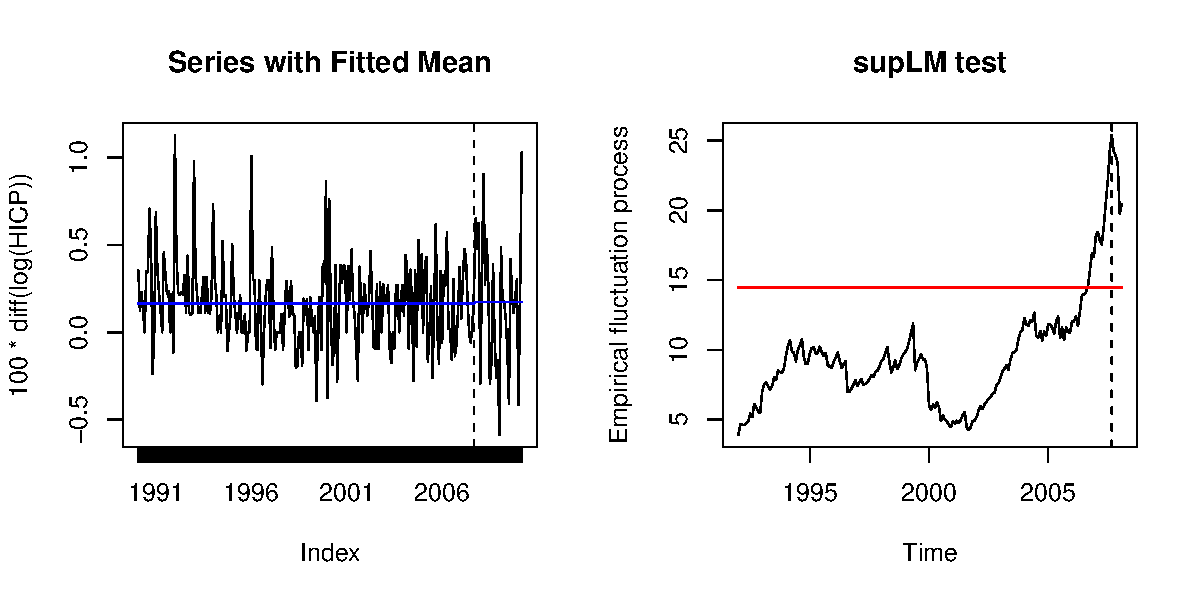
\includegraphics{results-012.pdf}
  \caption{Series and supLM test for Austria}
  \label{aut}
\end{figure}

The reason for this is a strong increase in the yearly Austrian inflation rate following a heavy increase in oil price which was further amplified by a rise of minearl taxes. However, we fail to find any evidence for an incrase in mean or volatility of the Austrian rate following the introduction of the Euro paper money. 

Let us consider Slovenia as the first Eastern European country that introduced the Euro. In August 2003 the new regime started with a much lower mean value (only a third now of its previous value) and interestingly enough, a higher volatility. 

\begin{figure}[ht!p]
  \centering
    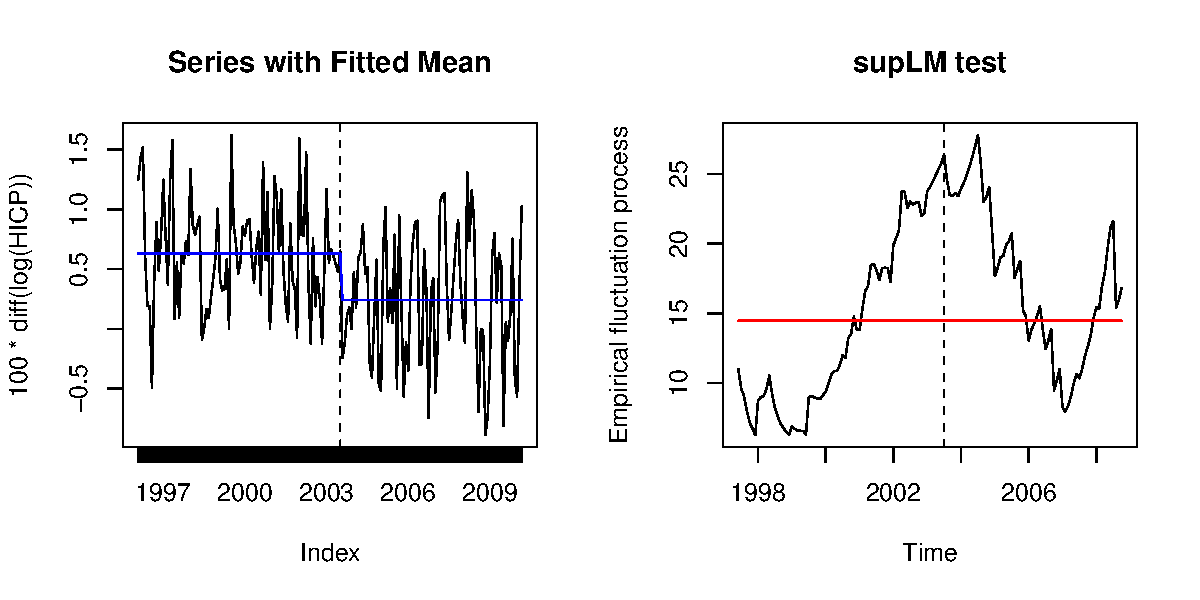
\includegraphics{results-131.pdf}
  \caption{Series and supLM test for Slovenia}
  \label{aut}
\end{figure}

%
%The LWZ criteria favors one break. 
%
%
%\begin{figure}[ht!p]
%  \centering
%    \includegraphics{results-132.pdf}
%  \caption{LWZ and Negative Log-Likelihood for Break Point Selection}
%  \label{aut}
%\end{figure}

Slovenia is a good example of the benefits of an early Euro adoption. Its efforts to meet the criterias as set forth in the Maastricht treaty were successfull, actually Slovenia reached them in 2005. So from 2003 onwards inflation was lower but with a much higher variance. Regarding the dating in 2003, we have to keep in mind that this was the year where most of the financial reforms were introduced. Slovenia seems to be the only case where the introduction of the Euro was followed by an increase in yearly inflation, which faded away following the financial crises and its deflationary effects. 

As a last example we focus on Spain. 

%The AR distances table, measuring the similarity of short--run inflation dynamics as in \citet{palomba} more or less supports this group building, although it is much more accurate. The similarity of the structural breaks thus is interesting topic for future research. 

%give the 3 most similar in AR distances: in Palomba Paper (table 2)
%
%Italy: Greece, France, Portugal
%Poland: Ireland, Spain, UK
%Sweden: Denmark, Netherlands, UK
%Netherlands: Sweden, UK, Portugal
%France: Italy, Greece, Belgium
%
%
%either support or not support group 1
%AR distance: the lower the more similar
%


\section{Conlcusion}


\bibliography{papers}


\end{document}
